% Options for packages loaded elsewhere
\PassOptionsToPackage{unicode}{hyperref}
\PassOptionsToPackage{hyphens}{url}
%
\documentclass[
]{article}
\usepackage{amsmath,amssymb}
\usepackage{lmodern}
\usepackage{iftex}
\ifPDFTeX
  \usepackage[T1]{fontenc}
  \usepackage[utf8]{inputenc}
  \usepackage{textcomp} % provide euro and other symbols
\else % if luatex or xetex
  \usepackage{unicode-math}
  \defaultfontfeatures{Scale=MatchLowercase}
  \defaultfontfeatures[\rmfamily]{Ligatures=TeX,Scale=1}
\fi
% Use upquote if available, for straight quotes in verbatim environments
\IfFileExists{upquote.sty}{\usepackage{upquote}}{}
\IfFileExists{microtype.sty}{% use microtype if available
  \usepackage[]{microtype}
  \UseMicrotypeSet[protrusion]{basicmath} % disable protrusion for tt fonts
}{}
\makeatletter
\@ifundefined{KOMAClassName}{% if non-KOMA class
  \IfFileExists{parskip.sty}{%
    \usepackage{parskip}
  }{% else
    \setlength{\parindent}{0pt}
    \setlength{\parskip}{6pt plus 2pt minus 1pt}}
}{% if KOMA class
  \KOMAoptions{parskip=half}}
\makeatother
\usepackage{xcolor}
\usepackage[margin=1in]{geometry}
\usepackage{color}
\usepackage{fancyvrb}
\newcommand{\VerbBar}{|}
\newcommand{\VERB}{\Verb[commandchars=\\\{\}]}
\DefineVerbatimEnvironment{Highlighting}{Verbatim}{commandchars=\\\{\}}
% Add ',fontsize=\small' for more characters per line
\usepackage{framed}
\definecolor{shadecolor}{RGB}{248,248,248}
\newenvironment{Shaded}{\begin{snugshade}}{\end{snugshade}}
\newcommand{\AlertTok}[1]{\textcolor[rgb]{0.94,0.16,0.16}{#1}}
\newcommand{\AnnotationTok}[1]{\textcolor[rgb]{0.56,0.35,0.01}{\textbf{\textit{#1}}}}
\newcommand{\AttributeTok}[1]{\textcolor[rgb]{0.77,0.63,0.00}{#1}}
\newcommand{\BaseNTok}[1]{\textcolor[rgb]{0.00,0.00,0.81}{#1}}
\newcommand{\BuiltInTok}[1]{#1}
\newcommand{\CharTok}[1]{\textcolor[rgb]{0.31,0.60,0.02}{#1}}
\newcommand{\CommentTok}[1]{\textcolor[rgb]{0.56,0.35,0.01}{\textit{#1}}}
\newcommand{\CommentVarTok}[1]{\textcolor[rgb]{0.56,0.35,0.01}{\textbf{\textit{#1}}}}
\newcommand{\ConstantTok}[1]{\textcolor[rgb]{0.00,0.00,0.00}{#1}}
\newcommand{\ControlFlowTok}[1]{\textcolor[rgb]{0.13,0.29,0.53}{\textbf{#1}}}
\newcommand{\DataTypeTok}[1]{\textcolor[rgb]{0.13,0.29,0.53}{#1}}
\newcommand{\DecValTok}[1]{\textcolor[rgb]{0.00,0.00,0.81}{#1}}
\newcommand{\DocumentationTok}[1]{\textcolor[rgb]{0.56,0.35,0.01}{\textbf{\textit{#1}}}}
\newcommand{\ErrorTok}[1]{\textcolor[rgb]{0.64,0.00,0.00}{\textbf{#1}}}
\newcommand{\ExtensionTok}[1]{#1}
\newcommand{\FloatTok}[1]{\textcolor[rgb]{0.00,0.00,0.81}{#1}}
\newcommand{\FunctionTok}[1]{\textcolor[rgb]{0.00,0.00,0.00}{#1}}
\newcommand{\ImportTok}[1]{#1}
\newcommand{\InformationTok}[1]{\textcolor[rgb]{0.56,0.35,0.01}{\textbf{\textit{#1}}}}
\newcommand{\KeywordTok}[1]{\textcolor[rgb]{0.13,0.29,0.53}{\textbf{#1}}}
\newcommand{\NormalTok}[1]{#1}
\newcommand{\OperatorTok}[1]{\textcolor[rgb]{0.81,0.36,0.00}{\textbf{#1}}}
\newcommand{\OtherTok}[1]{\textcolor[rgb]{0.56,0.35,0.01}{#1}}
\newcommand{\PreprocessorTok}[1]{\textcolor[rgb]{0.56,0.35,0.01}{\textit{#1}}}
\newcommand{\RegionMarkerTok}[1]{#1}
\newcommand{\SpecialCharTok}[1]{\textcolor[rgb]{0.00,0.00,0.00}{#1}}
\newcommand{\SpecialStringTok}[1]{\textcolor[rgb]{0.31,0.60,0.02}{#1}}
\newcommand{\StringTok}[1]{\textcolor[rgb]{0.31,0.60,0.02}{#1}}
\newcommand{\VariableTok}[1]{\textcolor[rgb]{0.00,0.00,0.00}{#1}}
\newcommand{\VerbatimStringTok}[1]{\textcolor[rgb]{0.31,0.60,0.02}{#1}}
\newcommand{\WarningTok}[1]{\textcolor[rgb]{0.56,0.35,0.01}{\textbf{\textit{#1}}}}
\usepackage{graphicx}
\makeatletter
\def\maxwidth{\ifdim\Gin@nat@width>\linewidth\linewidth\else\Gin@nat@width\fi}
\def\maxheight{\ifdim\Gin@nat@height>\textheight\textheight\else\Gin@nat@height\fi}
\makeatother
% Scale images if necessary, so that they will not overflow the page
% margins by default, and it is still possible to overwrite the defaults
% using explicit options in \includegraphics[width, height, ...]{}
\setkeys{Gin}{width=\maxwidth,height=\maxheight,keepaspectratio}
% Set default figure placement to htbp
\makeatletter
\def\fps@figure{htbp}
\makeatother
\setlength{\emergencystretch}{3em} % prevent overfull lines
\providecommand{\tightlist}{%
  \setlength{\itemsep}{0pt}\setlength{\parskip}{0pt}}
\setcounter{secnumdepth}{-\maxdimen} % remove section numbering
\ifLuaTeX
  \usepackage{selnolig}  % disable illegal ligatures
\fi
\IfFileExists{bookmark.sty}{\usepackage{bookmark}}{\usepackage{hyperref}}
\IfFileExists{xurl.sty}{\usepackage{xurl}}{} % add URL line breaks if available
\urlstyle{same} % disable monospaced font for URLs
\hypersetup{
  pdftitle={Chapter 4: Programming Fundamentals},
  pdfauthor={Ram Gopal, Dan Philps, and Tillman Weyde},
  hidelinks,
  pdfcreator={LaTeX via pandoc}}

\title{Chapter 4: Programming Fundamentals}
\author{Ram Gopal, Dan Philps, and Tillman Weyde}
\date{Summer 2022}

\begin{document}
\maketitle

{
\setcounter{tocdepth}{4}
\tableofcontents
}
In this lesson, we will explore some important programming constructs in
R.

\hypertarget{functions}{%
\section{Functions}\label{functions}}

Thus far, we have used many functions available in base R as well as in
packages that we have explored. Examples of these functions include
\texttt{mean()}, \texttt{std()}, \texttt{integrate}, and others. You can
create your own functions, as well. Let us do an example.

There is no function available in base R to compute geometric mean.
Geometric mean of positive numbers \(a_1\),\(a_2\),\ldots{}\(a_n\) is
defined as:\\
\[(a_1\times a_2\times a_3...a_n)^{1/n}\]\\
Now we will attempt to create a function ourselves. Before we do this,
let us write the code to compute the geometric mean of a set of numbers.

\begin{Shaded}
\begin{Highlighting}[]
\NormalTok{v }\OtherTok{=} \FunctionTok{c}\NormalTok{(}\DecValTok{1}\NormalTok{,}\DecValTok{33}\NormalTok{,}\DecValTok{4}\NormalTok{,}\DecValTok{29}\NormalTok{,}\DecValTok{9}\NormalTok{,}\DecValTok{90}\NormalTok{)}
\NormalTok{gmean }\OtherTok{=}\NormalTok{ (}\FunctionTok{prod}\NormalTok{(v))}\SpecialCharTok{\^{}}\NormalTok{(}\DecValTok{1}\SpecialCharTok{/}\FunctionTok{length}\NormalTok{(v))}
\NormalTok{gmean}
\end{Highlighting}
\end{Shaded}

\begin{verbatim}
## [1] 12.08
\end{verbatim}

The above code works fine to compute the geometric mean. What we would
like to do is package this into a function so it can be used repeatedly
in this script or others that we may write. This is the anatomy of a
function:\\
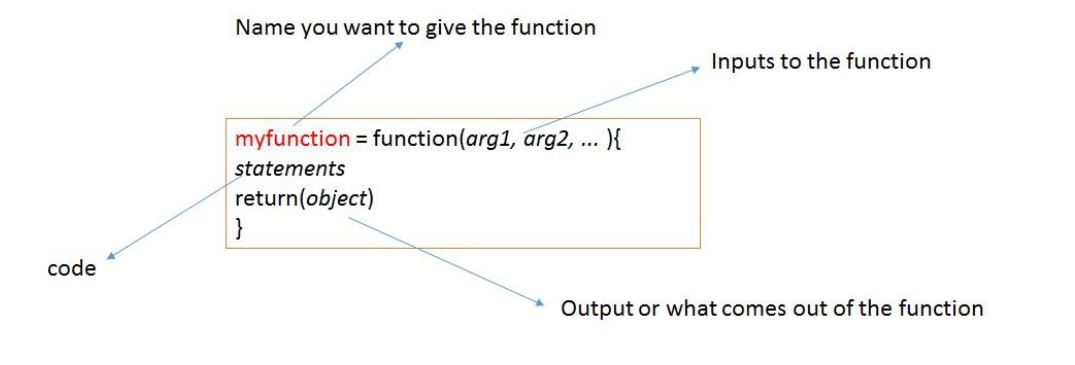
\includegraphics{FunctionPic.JPG}

\begin{Shaded}
\begin{Highlighting}[]
\NormalTok{geomean }\OtherTok{=} \ControlFlowTok{function}\NormalTok{(v)\{}
\NormalTok{gmean }\OtherTok{=}\NormalTok{ (}\FunctionTok{prod}\NormalTok{(v))}\SpecialCharTok{\^{}}\NormalTok{(}\DecValTok{1}\SpecialCharTok{/}\FunctionTok{length}\NormalTok{(v))}
\FunctionTok{return}\NormalTok{(gmean)}
\NormalTok{\}}
\end{Highlighting}
\end{Shaded}

That is how you create a function! Once the function is created, you can
send any input as a vector and our function will calculate the answer.
Here is an example of how we call the function.

\begin{Shaded}
\begin{Highlighting}[]
\NormalTok{x }\OtherTok{=} \FunctionTok{c}\NormalTok{(}\DecValTok{1}\NormalTok{,}\DecValTok{3}\NormalTok{,}\DecValTok{54}\NormalTok{,}\DecValTok{9}\NormalTok{,}\DecValTok{29}\NormalTok{,}\DecValTok{234}\NormalTok{,}\DecValTok{6}\NormalTok{,}\DecValTok{2}\NormalTok{,}\DecValTok{8}\NormalTok{,}\DecValTok{2456}\NormalTok{,}\DecValTok{2}\NormalTok{,}\DecValTok{8}\NormalTok{)}
\FunctionTok{geomean}\NormalTok{(x)}
\end{Highlighting}
\end{Shaded}

\begin{verbatim}
## [1] 13.52
\end{verbatim}

As another example, let us compute the harmonic mean which is defined
as:

\[{n}\over{{1\over{a_1}}+...+{1\over{a_n}}}\]

The following code will give us the harmonic mean.

\begin{Shaded}
\begin{Highlighting}[]
\NormalTok{d }\OtherTok{=} \FunctionTok{c}\NormalTok{(}\DecValTok{2}\NormalTok{,}\DecValTok{4}\NormalTok{,}\DecValTok{63}\NormalTok{,}\DecValTok{6}\NormalTok{,}\DecValTok{3}\NormalTok{)}
\NormalTok{g }\OtherTok{=} \DecValTok{1}\SpecialCharTok{/}\NormalTok{d}
\NormalTok{hmean }\OtherTok{=} \FunctionTok{length}\NormalTok{(d)}\SpecialCharTok{/}\NormalTok{(}\FunctionTok{sum}\NormalTok{(g))}
\NormalTok{hmean}
\end{Highlighting}
\end{Shaded}

\begin{verbatim}
## [1] 3.95
\end{verbatim}

Now, let us create a function for harmonic mean.

\begin{Shaded}
\begin{Highlighting}[]
\NormalTok{harmean }\OtherTok{=} \ControlFlowTok{function}\NormalTok{(v)\{}
\NormalTok{  a }\OtherTok{=} \DecValTok{1}\SpecialCharTok{/}\NormalTok{v}
\NormalTok{  hmean }\OtherTok{=} \FunctionTok{length}\NormalTok{(v)}\SpecialCharTok{/}\NormalTok{(}\FunctionTok{sum}\NormalTok{(a))}
  \FunctionTok{return}\NormalTok{(hmean)}
\NormalTok{\}}
\end{Highlighting}
\end{Shaded}

Now we will test both of the functions.

\begin{Shaded}
\begin{Highlighting}[]
\NormalTok{v }\OtherTok{=} \FunctionTok{c}\NormalTok{(}\DecValTok{2}\NormalTok{,}\DecValTok{23}\NormalTok{,}\DecValTok{3456}\NormalTok{,}\DecValTok{1}\NormalTok{,}\DecValTok{4}\NormalTok{,}\DecValTok{6}\NormalTok{)}
\FunctionTok{geomean}\NormalTok{(v)}
\end{Highlighting}
\end{Shaded}

\begin{verbatim}
## [1] 12.5
\end{verbatim}

\begin{Shaded}
\begin{Highlighting}[]
\FunctionTok{harmean}\NormalTok{(v)}
\end{Highlighting}
\end{Shaded}

\begin{verbatim}
## [1] 3.061
\end{verbatim}

Let us try another example. Suppose we have a vector
\(v = [4,6,23,6,375,9]\) and we want to find how many elements of the
vector are above a cutoff number, say 6. The following code can be used
to find this.

\begin{Shaded}
\begin{Highlighting}[]
\NormalTok{v }\OtherTok{=} \FunctionTok{c}\NormalTok{(}\DecValTok{4}\NormalTok{,}\DecValTok{6}\NormalTok{,}\DecValTok{23}\NormalTok{,}\DecValTok{6}\NormalTok{,}\DecValTok{375}\NormalTok{,}\DecValTok{9}\NormalTok{)}
\NormalTok{cutoff }\OtherTok{=} \DecValTok{6}
\NormalTok{vsub }\OtherTok{=}\NormalTok{ v[v}\SpecialCharTok{\textgreater{}}\NormalTok{cutoff]}
\NormalTok{vsub}
\end{Highlighting}
\end{Shaded}

\begin{verbatim}
## [1]  23 375   9
\end{verbatim}

\begin{Shaded}
\begin{Highlighting}[]
\FunctionTok{length}\NormalTok{(vsub)}
\end{Highlighting}
\end{Shaded}

\begin{verbatim}
## [1] 3
\end{verbatim}

Next, let us package this into a function. You should notice that this
function should have two inputs: the vector and the cutoff value.

\begin{Shaded}
\begin{Highlighting}[]
\NormalTok{vecsize }\OtherTok{=} \ControlFlowTok{function}\NormalTok{(v,}\AttributeTok{cutoff =} \DecValTok{1}\NormalTok{)\{}
\NormalTok{  vsub }\OtherTok{=}\NormalTok{ v[v}\SpecialCharTok{\textgreater{}}\NormalTok{cutoff]}
  \FunctionTok{return}\NormalTok{(}\FunctionTok{length}\NormalTok{(vsub))}
\NormalTok{\}}
\end{Highlighting}
\end{Shaded}

Let us see how this function works.

\begin{Shaded}
\begin{Highlighting}[]
\NormalTok{v }\OtherTok{=} \FunctionTok{c}\NormalTok{(.}\DecValTok{2}\NormalTok{,}\DecValTok{5}\NormalTok{,}\DecValTok{2}\NormalTok{,.}\DecValTok{6}\NormalTok{,}\DecValTok{3}\NormalTok{,}\DecValTok{57}\NormalTok{,}\DecValTok{34}\NormalTok{,}\DecValTok{5}\NormalTok{)}
\FunctionTok{vecsize}\NormalTok{(v,}\DecValTok{10}\NormalTok{)}
\end{Highlighting}
\end{Shaded}

\begin{verbatim}
## [1] 2
\end{verbatim}

You will notice that in the function, we have set a default cutoff value
of 1 by using \texttt{cutoff\ =\ 1}. If you do not specify a cutoff
value when using the function, it defaults to 1. For example

\begin{Shaded}
\begin{Highlighting}[]
\FunctionTok{vecsize}\NormalTok{(v)}
\end{Highlighting}
\end{Shaded}

\begin{verbatim}
## [1] 6
\end{verbatim}

Let us do another example. Suppose we have a vector
\(v = [2,2,6,3,546,2346,22,34,7,21,4]\) and we want to see all the
elements between 5 and 100. The following code can be used to find this.

\begin{Shaded}
\begin{Highlighting}[]
\NormalTok{vec1 }\OtherTok{=} \FunctionTok{c}\NormalTok{(}\DecValTok{2}\NormalTok{,}\DecValTok{2}\NormalTok{,}\DecValTok{6}\NormalTok{,}\DecValTok{3}\NormalTok{,}\DecValTok{546}\NormalTok{,}\DecValTok{2346}\NormalTok{,}\DecValTok{22}\NormalTok{,}\DecValTok{34}\NormalTok{,}\DecValTok{7}\NormalTok{,}\DecValTok{21}\NormalTok{,}\DecValTok{4}\NormalTok{)}
\NormalTok{cutoff1 }\OtherTok{=} \DecValTok{5}
\NormalTok{cutoff2 }\OtherTok{=} \DecValTok{100} 
\NormalTok{vsub }\OtherTok{=}\NormalTok{ vec1[vec1}\SpecialCharTok{\textgreater{}}\NormalTok{cutoff1 }\SpecialCharTok{\&}\NormalTok{ vec1}\SpecialCharTok{\textless{}}\NormalTok{cutoff2]}
\NormalTok{vsub}
\end{Highlighting}
\end{Shaded}

\begin{verbatim}
## [1]  6 22 34  7 21
\end{verbatim}

Now, let us turn this into a function.

\begin{Shaded}
\begin{Highlighting}[]
\NormalTok{Intermediate }\OtherTok{=} \ControlFlowTok{function}\NormalTok{(vec1, cutoff1, cutoff2)\{}
\NormalTok{  vsub }\OtherTok{=}\NormalTok{ vec1[vec1}\SpecialCharTok{\textgreater{}}\NormalTok{cutoff1 }\SpecialCharTok{\&}\NormalTok{ vec1}\SpecialCharTok{\textless{}}\NormalTok{cutoff2]}
  \FunctionTok{return}\NormalTok{(vsub)}
\NormalTok{\}}
\end{Highlighting}
\end{Shaded}

Let us see how this works.

\begin{Shaded}
\begin{Highlighting}[]
\NormalTok{vec1 }\OtherTok{=} \FunctionTok{c}\NormalTok{(}\DecValTok{2}\NormalTok{,}\DecValTok{2}\NormalTok{,}\DecValTok{6}\NormalTok{,}\DecValTok{3}\NormalTok{,}\DecValTok{546}\NormalTok{,}\DecValTok{2346}\NormalTok{,}\DecValTok{22}\NormalTok{,}\DecValTok{34}\NormalTok{,}\DecValTok{7}\NormalTok{,}\DecValTok{21}\NormalTok{,}\DecValTok{4}\NormalTok{)}
\FunctionTok{Intermediate}\NormalTok{(vec1,}\DecValTok{5}\NormalTok{,}\DecValTok{100}\NormalTok{)}
\end{Highlighting}
\end{Shaded}

\begin{verbatim}
## [1]  6 22 34  7 21
\end{verbatim}

\hypertarget{conditional-statements}{%
\section{Conditional Statements}\label{conditional-statements}}

Conditional statements are very useful and are an important element to
any programming language. There are three varieties of syntax for
conditional statements in R:

\begin{enumerate}
\def\labelenumi{\arabic{enumi}.}
\tightlist
\item
  \texttt{if\ (condition)\ \{trueExpressions\}}
\item
  \texttt{ifelse\ (condition,trueExpressions,falseExpressions)}
\item
  \texttt{if\ (condition)\{trueExpressions\}\ else\ \{falseExpressions\}}
\end{enumerate}

Suppose we have a vector of numbers and we want to create another vector
containing 0s and 1s. If the element in the first vector is 5 or above,
we want to put a 1 for the corresponding element in the second vector.
Otherwise, we want to put a 0. The appropriate code in R is

\begin{Shaded}
\begin{Highlighting}[]
\NormalTok{v1 }\OtherTok{=} \FunctionTok{c}\NormalTok{(}\DecValTok{2}\NormalTok{,}\DecValTok{36}\NormalTok{,}\DecValTok{83}\NormalTok{,}\DecValTok{2}\NormalTok{,}\DecValTok{5}\NormalTok{,}\DecValTok{7}\NormalTok{,}\DecValTok{2}\NormalTok{,}\DecValTok{9}\NormalTok{,}\DecValTok{3}\NormalTok{,}\DecValTok{12}\NormalTok{)}
\NormalTok{v2 }\OtherTok{=} \FunctionTok{ifelse}\NormalTok{(v1}\SpecialCharTok{\textgreater{}=}\DecValTok{5}\NormalTok{,}\DecValTok{1}\NormalTok{,}\DecValTok{0}\NormalTok{)}
\FunctionTok{print}\NormalTok{(v2)}
\end{Highlighting}
\end{Shaded}

\begin{verbatim}
##  [1] 0 1 1 0 1 1 0 1 0 1
\end{verbatim}

Let us do another example. In the \texttt{MASS} package, there is a data
frame called \texttt{whiteside}. Let us take a look at it.

\begin{Shaded}
\begin{Highlighting}[]
\FunctionTok{library}\NormalTok{(MASS)}
\FunctionTok{head}\NormalTok{(whiteside)}
\end{Highlighting}
\end{Shaded}

\begin{verbatim}
##    Insul Temp Gas
## 1 Before -0.8 7.2
## 2 Before -0.7 6.9
## 3 Before  0.4 6.4
## 4 Before  2.5 6.0
## 5 Before  2.9 5.8
## 6 Before  3.2 5.8
\end{verbatim}

Suppose we want to create a column in which temperatures below 5 are
labeled cold and temperatures above 5 are labeled hot.

\begin{Shaded}
\begin{Highlighting}[]
\NormalTok{whiteside}\SpecialCharTok{$}\NormalTok{hotcold }\OtherTok{=} \FunctionTok{ifelse}\NormalTok{(whiteside}\SpecialCharTok{$}\NormalTok{Temp}\SpecialCharTok{\textless{}}\DecValTok{5}\NormalTok{,}\StringTok{"cold"}\NormalTok{,}\StringTok{"hot"}\NormalTok{)}
\FunctionTok{head}\NormalTok{(whiteside)}
\end{Highlighting}
\end{Shaded}

\begin{verbatim}
##    Insul Temp Gas hotcold
## 1 Before -0.8 7.2    cold
## 2 Before -0.7 6.9    cold
## 3 Before  0.4 6.4    cold
## 4 Before  2.5 6.0    cold
## 5 Before  2.9 5.8    cold
## 6 Before  3.2 5.8    cold
\end{verbatim}

Next, let us create a summary table of average gas consumption when it
is hot and cold, and with and without insulation. As before, we use the
\texttt{aggregate()} function to summarize.

\begin{Shaded}
\begin{Highlighting}[]
\NormalTok{x }\OtherTok{=} \FunctionTok{aggregate}\NormalTok{(whiteside}\SpecialCharTok{$}\NormalTok{Gas,}\FunctionTok{list}\NormalTok{(whiteside}\SpecialCharTok{$}\NormalTok{Insul, whiteside}\SpecialCharTok{$}\NormalTok{hotcold),mean)}
\NormalTok{x}
\end{Highlighting}
\end{Shaded}

\begin{verbatim}
##   Group.1 Group.2     x
## 1  Before    cold 5.940
## 2   After    cold 3.885
## 3  Before     hot 4.006
## 4   After     hot 2.680
\end{verbatim}

It works well! As expected, gas consumption is high when it is cold and
when there is no insulation. Notice that the column names are not very
informative. The column names of a data frame can be changed using the
\texttt{colnames()} function.

\begin{Shaded}
\begin{Highlighting}[]
\FunctionTok{colnames}\NormalTok{(x)}
\end{Highlighting}
\end{Shaded}

\begin{verbatim}
## [1] "Group.1" "Group.2" "x"
\end{verbatim}

\begin{Shaded}
\begin{Highlighting}[]
\FunctionTok{colnames}\NormalTok{(x) }\OtherTok{=} \FunctionTok{c}\NormalTok{(}\StringTok{"Insulation"}\NormalTok{,}\StringTok{"Weather"}\NormalTok{, }\StringTok{"Average\_Gas\_Consumption"}\NormalTok{)}
\NormalTok{x}
\end{Highlighting}
\end{Shaded}

\begin{verbatim}
##   Insulation Weather Average_Gas_Consumption
## 1     Before    cold                   5.940
## 2      After    cold                   3.885
## 3     Before     hot                   4.006
## 4      After     hot                   2.680
\end{verbatim}

\hypertarget{looping}{%
\section{Looping}\label{looping}}

\hypertarget{for-loops}{%
\subsection{For Loops}\label{for-loops}}

Looping or iterations is another key element of programming. The syntax
is as follows:

\texttt{for\ (var\ in\ seq)\ \{statements\}}

It is common to use \texttt{i} as the variable in the sequence. The
command \texttt{print} allows you to write things out from inside the
loop.

Let us try an example. Say that you want to print the numbers 1-10 using
a loop.

\begin{Shaded}
\begin{Highlighting}[]
\ControlFlowTok{for}\NormalTok{ (i }\ControlFlowTok{in} \DecValTok{1}\SpecialCharTok{:}\DecValTok{10}\NormalTok{)}
\NormalTok{\{}
  \FunctionTok{print}\NormalTok{(i)}
\NormalTok{\}}
\end{Highlighting}
\end{Shaded}

\begin{verbatim}
## [1] 1
## [1] 2
## [1] 3
## [1] 4
## [1] 5
## [1] 6
## [1] 7
## [1] 8
## [1] 9
## [1] 10
\end{verbatim}

Next, let us say you want to print the product of a term and the two
terms before it. The code would be as follows:

\begin{Shaded}
\begin{Highlighting}[]
\ControlFlowTok{for}\NormalTok{ (i }\ControlFlowTok{in} \DecValTok{1}\SpecialCharTok{:}\DecValTok{10}\NormalTok{)}
\NormalTok{\{}
  \FunctionTok{print}\NormalTok{(i}\SpecialCharTok{*}\NormalTok{(i}\DecValTok{{-}1}\NormalTok{)}\SpecialCharTok{*}\NormalTok{(i}\DecValTok{{-}2}\NormalTok{))}
\NormalTok{\}}
\end{Highlighting}
\end{Shaded}

\begin{verbatim}
## [1] 0
## [1] 0
## [1] 6
## [1] 24
## [1] 60
## [1] 120
## [1] 210
## [1] 336
## [1] 504
## [1] 720
\end{verbatim}

Now, let us say you want a vector that gives you the running sums the
elements in vector \(v1 = [1,2,4,2,4,6,7,8,9,12,4,1,5,2]\). The code can
be written as follows:

\begin{Shaded}
\begin{Highlighting}[]
\NormalTok{v1 }\OtherTok{=} \FunctionTok{c}\NormalTok{(}\DecValTok{1}\NormalTok{,}\DecValTok{4}\NormalTok{,}\DecValTok{5}\NormalTok{,}\DecValTok{2}\NormalTok{,}\DecValTok{4}\NormalTok{,}\DecValTok{6}\NormalTok{,}\DecValTok{7}\NormalTok{,}\DecValTok{8}\NormalTok{,}\DecValTok{9}\NormalTok{,}\DecValTok{12}\NormalTok{,}\DecValTok{4}\NormalTok{,}\DecValTok{1}\NormalTok{,}\DecValTok{5}\NormalTok{,}\DecValTok{2}\NormalTok{)}
\NormalTok{v2 }\OtherTok{=}\NormalTok{ v1}
\ControlFlowTok{for}\NormalTok{ (i }\ControlFlowTok{in} \DecValTok{2}\SpecialCharTok{:}\FunctionTok{length}\NormalTok{(v1))}
\NormalTok{\{}
\NormalTok{  v2[i]}\OtherTok{=}\NormalTok{v2[i}\DecValTok{{-}1}\NormalTok{]}\SpecialCharTok{+}\NormalTok{v1[i]}
\NormalTok{\}}
\NormalTok{v2}
\end{Highlighting}
\end{Shaded}

\begin{verbatim}
##  [1]  1  5 10 12 16 22 29 37 46 58 62 63 68 70
\end{verbatim}

For the next example, we want to create a vector that gives you all the
prime numbers between two integers of your choice. To do this, you will
need to install the package \texttt{schoolmath}.

\begin{Shaded}
\begin{Highlighting}[]
\FunctionTok{library}\NormalTok{(schoolmath)}
\NormalTok{ans }\OtherTok{=} \FunctionTok{c}\NormalTok{()}
\NormalTok{a }\OtherTok{=} \DecValTok{20}
\NormalTok{b }\OtherTok{=} \DecValTok{30}
\ControlFlowTok{for}\NormalTok{ (i }\ControlFlowTok{in}\NormalTok{ a}\SpecialCharTok{:}\NormalTok{b)}
\NormalTok{\{}
  \ControlFlowTok{if}\NormalTok{(}\FunctionTok{is.prim}\NormalTok{(i)}\SpecialCharTok{==}\ConstantTok{TRUE}\NormalTok{)\{ans }\OtherTok{=} \FunctionTok{c}\NormalTok{(ans,i)\}}
\NormalTok{\}}
\NormalTok{ans}
\end{Highlighting}
\end{Shaded}

\begin{verbatim}
## [1] 23 29
\end{verbatim}

\hypertarget{avoiding-loops}{%
\subsection{Avoiding Loops}\label{avoiding-loops}}

Even though we wrote the above code using loops, we won't necessarily
have to use loops in R. This is because R does vectorized calculations.
This makes it easy to code without having to write loops many times. For
example, when we did the sum of a vector, to add up all the numbers, we
used \texttt{sum()}. In other programming languages which do not support
vectorized calculations, you will have to write a loop to calculate the
sum of the numbers in a vector. In general, use vectorized calculations
and try to avoid using loops.

Now, we will rewrite the above code above without using a loop.

\begin{Shaded}
\begin{Highlighting}[]
\NormalTok{x }\OtherTok{=} \FunctionTok{seq}\NormalTok{(}\DecValTok{20}\SpecialCharTok{:}\DecValTok{30}\NormalTok{)}
\NormalTok{y }\OtherTok{=} \FunctionTok{is.prim}\NormalTok{(x)}
\NormalTok{y}
\end{Highlighting}
\end{Shaded}

\begin{verbatim}
##  [1]  TRUE  TRUE  TRUE FALSE  TRUE FALSE  TRUE FALSE FALSE FALSE  TRUE
\end{verbatim}

\begin{Shaded}
\begin{Highlighting}[]
\NormalTok{x[y]}
\end{Highlighting}
\end{Shaded}

\begin{verbatim}
## [1]  1  2  3  5  7 11
\end{verbatim}

If you compare the two chunks of code, you will see that writing the
code without using loops is much simpler and more elegant.

Now, suppose you have a vector \([a_1, a_2,...a_n]\) and you want to
calculate the following:\\
\[\sum_{i = 1}^{n-1} a_ia_{i+1}\]

\begin{Shaded}
\begin{Highlighting}[]
\NormalTok{total }\OtherTok{=} \DecValTok{0}
\NormalTok{v }\OtherTok{=} \FunctionTok{c}\NormalTok{(}\DecValTok{1}\NormalTok{,}\DecValTok{4}\NormalTok{,}\DecValTok{2}\NormalTok{,}\DecValTok{5}\NormalTok{,}\DecValTok{73}\NormalTok{,}\DecValTok{4}\NormalTok{,}\DecValTok{5}\NormalTok{)}
\ControlFlowTok{for}\NormalTok{ (i }\ControlFlowTok{in} \DecValTok{1}\SpecialCharTok{:}\NormalTok{(}\FunctionTok{length}\NormalTok{(v)}\SpecialCharTok{{-}}\DecValTok{1}\NormalTok{))}
\NormalTok{\{}
\NormalTok{  total }\OtherTok{=}\NormalTok{ total }\SpecialCharTok{+}\NormalTok{ (v[i]}\SpecialCharTok{*}\NormalTok{v[i}\SpecialCharTok{+}\DecValTok{1}\NormalTok{]) }
\NormalTok{\}}
\NormalTok{total}
\end{Highlighting}
\end{Shaded}

\begin{verbatim}
## [1] 699
\end{verbatim}

Again, there is a clever way to calculate this total without using loops
by creating vectors \(v1 = [a_1, a_2...,a_{n-1}]\) and
\(v2 = [a_2, a_3, ...,a_n]\). The code is:

\begin{Shaded}
\begin{Highlighting}[]
\NormalTok{v1 }\OtherTok{=}\NormalTok{ v[}\DecValTok{1}\SpecialCharTok{:}\NormalTok{(}\FunctionTok{length}\NormalTok{(v)}\SpecialCharTok{{-}}\DecValTok{1}\NormalTok{)] }
\NormalTok{v2 }\OtherTok{=}\NormalTok{ v[}\DecValTok{2}\SpecialCharTok{:}\FunctionTok{length}\NormalTok{(v)]}
\NormalTok{total }\OtherTok{=} \FunctionTok{sum}\NormalTok{(v1}\SpecialCharTok{*}\NormalTok{v2) }
\NormalTok{total}
\end{Highlighting}
\end{Shaded}

\begin{verbatim}
## [1] 699
\end{verbatim}

In some cases, you will have no option but to create a loop. Here is an
example.

Let us say you have a vector \(v1 = [1,2,3,4,5]\) and you want a loop
that flips the order of the elements in the vector.

\begin{Shaded}
\begin{Highlighting}[]
\NormalTok{v1 }\OtherTok{=} \FunctionTok{c}\NormalTok{(}\DecValTok{72}\NormalTok{,}\DecValTok{3}\NormalTok{,}\DecValTok{57}\NormalTok{,}\DecValTok{2}\NormalTok{,}\DecValTok{8}\NormalTok{,}\DecValTok{24}\NormalTok{,}\DecValTok{7}\NormalTok{)}
\NormalTok{v2 }\OtherTok{=} \FunctionTok{c}\NormalTok{()}
\NormalTok{n }\OtherTok{=} \FunctionTok{length}\NormalTok{(v1)}
\ControlFlowTok{for}\NormalTok{ (i }\ControlFlowTok{in} \DecValTok{1}\SpecialCharTok{:}\NormalTok{n)}
\NormalTok{\{}
\NormalTok{  v2[i] }\OtherTok{=}\NormalTok{ v1[n }\SpecialCharTok{+}\DecValTok{1} \SpecialCharTok{{-}}\NormalTok{ i]}
\NormalTok{\}}
\NormalTok{v2}
\end{Highlighting}
\end{Shaded}

\begin{verbatim}
## [1]  7 24  8  2 57  3 72
\end{verbatim}

I don't believe you can't do this without writing a loop, but if you
figure it out, let me know!

\hypertarget{while-loops}{%
\subsection{While Loops}\label{while-loops}}

Another type of iteration is the \texttt{while} loop. The syntax in R
is\\
\texttt{while(cond)\ expr}

The while loop is used when you want to repeat a set of commands while a
condition remains true.

Suppose you have a starting integer value, let us say 19. Now suppose
you want to find ten prime numbers that follow 19. For this, the
\texttt{for} loop is not useful. The logic to create this is as follows.

We will create one index called \texttt{i} that starts at 19 and will
increment by 1 at each iteration. We will create another index
\texttt{primi} which starts at 0 and will increment by 1 if a prime
number is found. The while loop will continue until \texttt{primi}
reaches 10.

\begin{Shaded}
\begin{Highlighting}[]
\FunctionTok{library}\NormalTok{(schoolmath)}
\NormalTok{startnumber }\OtherTok{=} \DecValTok{300}
\NormalTok{numprimes }\OtherTok{=} \DecValTok{3}
\NormalTok{i }\OtherTok{=}\NormalTok{ startnumber }\SpecialCharTok{+} \DecValTok{1}
\NormalTok{primi }\OtherTok{=} \DecValTok{0}
\NormalTok{primevec}\OtherTok{=} \FunctionTok{c}\NormalTok{()}
\ControlFlowTok{while}\NormalTok{ (primi}\SpecialCharTok{\textless{}}\NormalTok{numprimes)}
\NormalTok{\{}
  \ControlFlowTok{if}\NormalTok{(}\FunctionTok{is.prim}\NormalTok{(i)}\SpecialCharTok{==}\ConstantTok{TRUE}\NormalTok{)\{}
\NormalTok{    primi }\OtherTok{=}\NormalTok{ primi }\SpecialCharTok{+} \DecValTok{1}
\NormalTok{    primevec }\OtherTok{=} \FunctionTok{c}\NormalTok{(primevec,i)}
\NormalTok{    \}}
\NormalTok{  i }\OtherTok{=}\NormalTok{ i }\SpecialCharTok{+}\DecValTok{1}
\NormalTok{\}}
\FunctionTok{print}\NormalTok{(primevec)}
\end{Highlighting}
\end{Shaded}

\begin{verbatim}
## [1] 307 311 313
\end{verbatim}

Let us package this into a function.

\begin{Shaded}
\begin{Highlighting}[]
\NormalTok{nextprimes }\OtherTok{=} \ControlFlowTok{function}\NormalTok{(startnumber, numprimes)\{}
\NormalTok{  primi }\OtherTok{=} \DecValTok{0}
\NormalTok{  i }\OtherTok{=}\NormalTok{ startnumber }\SpecialCharTok{+} \DecValTok{1}
\NormalTok{  primevec }\OtherTok{=} \FunctionTok{c}\NormalTok{()}
  \ControlFlowTok{while}\NormalTok{ (primi}\SpecialCharTok{\textless{}}\NormalTok{numprimes)}
\NormalTok{  \{}
    \ControlFlowTok{if}\NormalTok{(}\FunctionTok{is.prim}\NormalTok{(i)}\SpecialCharTok{==}\ConstantTok{TRUE}\NormalTok{)\{}
\NormalTok{      primi }\OtherTok{=}\NormalTok{ primi }\SpecialCharTok{+} \DecValTok{1}
\NormalTok{      primevec }\OtherTok{=} \FunctionTok{c}\NormalTok{(primevec,i)}
\NormalTok{    \}}
\NormalTok{  i }\OtherTok{=}\NormalTok{ i }\SpecialCharTok{+}\DecValTok{1}
\NormalTok{  \}}
  \FunctionTok{return}\NormalTok{(}\FunctionTok{print}\NormalTok{(primevec))}
\NormalTok{\}}
\end{Highlighting}
\end{Shaded}

Now, let us test the function.

\begin{Shaded}
\begin{Highlighting}[]
\FunctionTok{nextprimes}\NormalTok{(}\DecValTok{3}\NormalTok{,}\DecValTok{3}\NormalTok{)}
\end{Highlighting}
\end{Shaded}

\begin{verbatim}
## [1]  5  7 11
\end{verbatim}

\begin{Shaded}
\begin{Highlighting}[]
\FunctionTok{nextprimes}\NormalTok{(}\DecValTok{19}\NormalTok{,}\DecValTok{10}\NormalTok{)}
\end{Highlighting}
\end{Shaded}

\begin{verbatim}
##  [1] 23 29 31 37 41 43 47 53 59 61
\end{verbatim}

\begin{Shaded}
\begin{Highlighting}[]
\FunctionTok{nextprimes}\NormalTok{(}\DecValTok{9}\NormalTok{,}\DecValTok{3}\NormalTok{)}
\end{Highlighting}
\end{Shaded}

\begin{verbatim}
## [1] 11 13 17
\end{verbatim}

It works!

In this lesson, we covered core programming elements in R. These come in
handy as you explore and do more with R. You will see these used
frequently in the coming set of lessons.

\end{document}
